
\title{Improving the Robustness of Human Pose Estimation using Fault Estimation on Multi-Modal Data}
\author{Leonardo Benedikt Pohl}
% TITLE
\date{\today}
 
\newlength{\originalVOffset}
\newlength{\originalHOffset}
\setlength{\originalVOffset}{\voffset}   
\setlength{\originalHOffset}{\hoffset}

\setlength{\voffset}{0cm}
\setlength{\hoffset}{0cm}
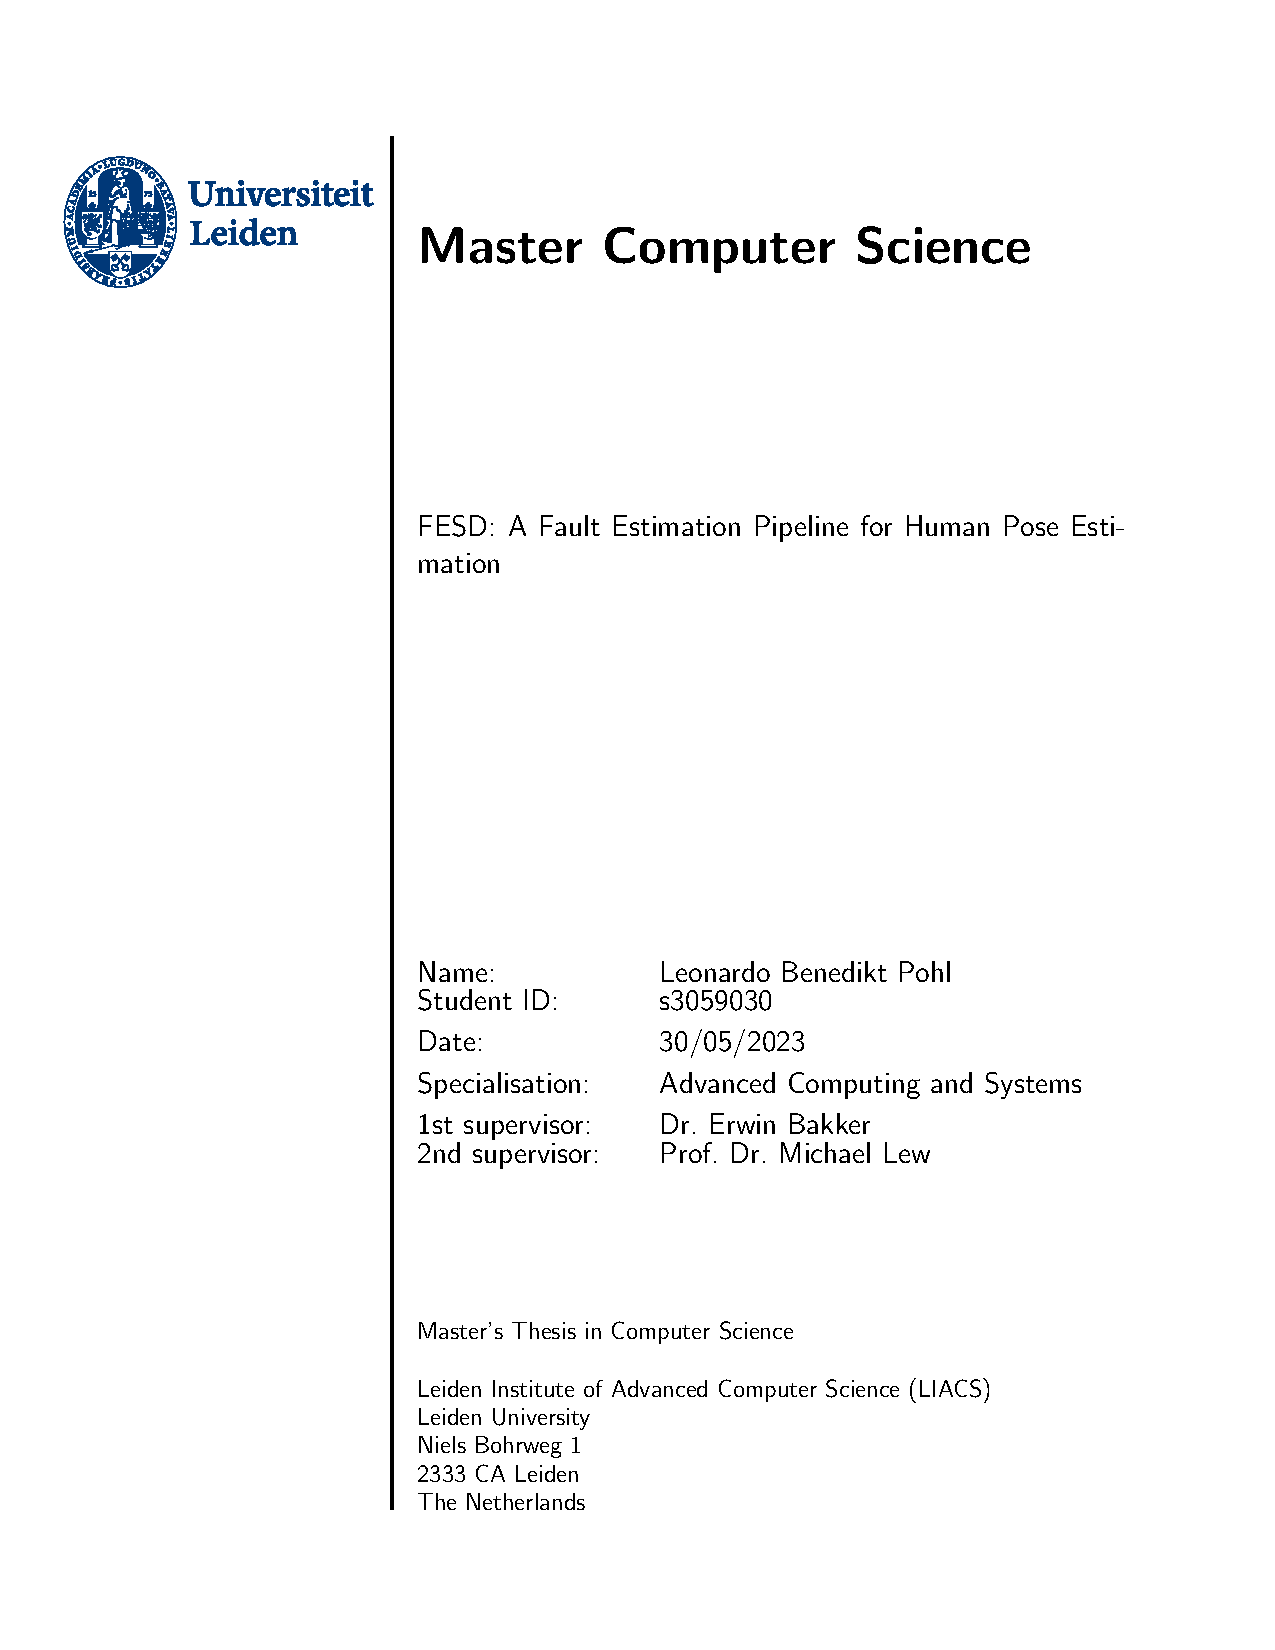
\includepdf[pages=1]{title_page.pdf}
\setlength{\voffset}{\originalVOffset}
\setlength{\hoffset}{\originalHOffset}

\clearpage

\begin{abstract}
  Human pose estimation(HPE), or skeleton detection, has been a topic of research for many years. With the advancement of hardware, it has become viable to apply HPE in real-time applications such as games. However, HPE is a difficult task that is prone to errors, especially in complicated situations, such as cramped environments. These errors might cause human-computer interaction to be hampered.

  The goal of this thesis is to obtain a better understanding of what causes the problems in HPE. Therefore, various exercises and scenarios are designed that exhibit common errors in HPE. The exercises are captured in a labelled dataset. Finally, preliminary models are developed and trained on the new dataset to automatically detect the HPE errors.

  The dataset is captured using a newly developed tool In this work, a tool is developed that is capable of capturing and labelling multi-modal data, the \textbf{F}ault \textbf{E}stimator for \textbf{S}keleton \textbf{D}etection \textbf{Data} (FESDData) tool. Four different datasets are captured using four problem sets with varying granularity, ranging from body-wise fault estimation to joint-wise fault estimation. Using the captured dataset, the FESDDataset, preliminary experiments were conducted using two new deep neural networks (DNNs), \textbf{F}ault \textbf{E}stimator for \textbf{S}keleton \textbf{D}etection \textbf{Model} V1 (FESDModelv1) and FESDModelv2. Where FESDModelv1 uses custom feature extraction, and FESDModelv2 uses transfer learning using EfficientNetv2.

  Preliminary experimental results showed promising performance of both FESDModelv1 and FESDModelv2 on coarse grain scenarios such as Half Body HPE error detection.

  % In this thesis, common error sources that occur during HPE are found. Based on these error sources, exercises are derived which are captured in the FESDDataset using the dataset collection tool FESDData. The joints of the poses are then labelled based on the errors that occur. I abstract the data to form four different problem sets. For each of the problem sets, two models FESDModelv1 and FESDModelv2, are trained. The results of 
  
  % The preliminary experiments showed that FESDModelv1 reaches the best F1-Score of the two models. Specifically, when trained on images with a resolution of 64x64 pixels on the Half Body problem set it achieves an F1-Score of $0.77$. FESDModelv2 achieved the best F1-Score of $0.71$ on the same problem set however, it achieves better results on higher resolution image with a resolution of 200x200 pixels.

% Given the results it is shown that the datasets captured by FESDData were useful to conduct research on fault estimation for skeleton detection and fault estimation for human pose estimation is possible using convolutional neural networks.

\end{abstract}
